\documentclass[a4paper,12pt,twoside]{book}

\usepackage{praca_dyplomowa}

\author{Michał Sośnicki}
\title{Usprawnienie programowania z~użyciem typów w~Glasgow Haskell Compiler}

\begin{document}
\frontmatter
\begin{titlepage}

\noindent
\begin{minipage}{0.19\textwidth}
\begin{flushleft}

\includegraphics[width=0.88\textwidth]{images/logo}
\end{flushleft}
\end{minipage}
\begin{minipage}[t][][t]{0.81\textwidth}
\begin{flushleft}
\vspace{-3.5\baselineskip}
\textbf{{\large Politechnika Łódzka}\\}
\vspace{\medskipamount}
\textbf{\large Wydział Fizyki Technicznej, Informatyki\\i~Matematyki Stosowanej}
\vspace{\medskipamount}\\
Instytut Informatyki
\\
Kierunek: Informatyka
\\
Specjalność: Sztuczna Inteligencja i Inżynieria Oprogramowania
\\
\end{flushleft}
\end{minipage}
\vspace{2.5cm}

\begin{center}
{\Large inż. Michał Sośnicki\\nr albumu 207597\\}
\vspace{2cm}
{\huge Rozpoznawanie mówcy zależne od tekstu \\z wykorzystaniem sieci neuronowych}
\end{center}
\vspace{3cm}
\hfill
\begin{minipage}{.55\columnwidth}
Praca magisterska\\
napisana pod kierunkiem\\
dr inż. Bartłomieja Stasiaka
\end{minipage}
\vfill
\begin{center}
Łódź 2018
\end{center}
\end{titlepage}

\tableofcontents

\mainmatter
\pagestyle{headings}
\chapter{Wstęp}\label{chap:wstep}

Zakresem niniejszej pracy magisterskiej są systemy rozpoznawania mówcy zależne od tekstu. Celem
pracy jest zbadanie możliwości wykorzystania modelu sieci neuronowej do rozwiązania tego problemu.

Rozpoznawanie mówcy polega na analizie nagrań dźwiękowych mowy w celu wydobycia cech biometrycznych
charakteryzujących osobę mówiącą. Wyróżnia się dwa praktyczne problemy do rozwiązania z wykorzystaniem tych
cech: problem weryfikacji mówcy oraz problem identyfikacji mówcy.

Weryfikacja mówcy polega na stwierdzeniu, czy nagranie pochodzi od pewnej zarejestrowanej wcześniej osoby
lub wykryciu, że jest na nim ktoś inny. Ten przypadek występuje na przykład przy uwierzytelnianiu za pomocą głosu
do systemu bankowego. Konieczne jest wtedy wykrycie, gdy oszust podaje się za prawdziwego właściciela konta.
Identyfikacja mówcy polega na rozpoznaniu, która z zarejestrowanych osób jest na nagraniu lub czy
jest na nim ktoś niezarejestrowany. Identyfikacja może być wykorzystana przez służby policyjne do
zidentyfikowania osób na zdobytym nagraniu.

Rozpoznawanie mówcy można również podzielić ze względu na to, czy treść nagrania jest znana z góry
na rozpoznawanie mówcy zależne od tekstu i niezależne od tekstu. Weryfikacja mówcy zwykle może
być przeprowadzona zależnie od tekstu, gdyż w typowych zastosowaniach można oczekiwać od weryfikowanej
osoby kooperacji. Znajomość treści jest cenna, gdyż pozwala zwiększyć skuteczność, szczególnie w sytuacji,
gdy nagrań rejestrujących jest tylko kilka\cite{parallelSpeakerAnd}. W przypadku,
gdy nagranie nie zawiera oczekiwanej treści
akceptowalne jest odrzucenie weryfikowanego nagrania niezależnie od mówcy.
Identyfikację z kolei trzeba przeprowadzać bez założeń co do treści nagrania, gdyż nagrywane osoby mogą
być tego nieświadome.
% cite że poprawia skuteczność jak mało nagrań

Jako że przedmiotem pracy jest rozpoznawanie mówcy zależne od tekstu, uwaga zostanie poświęcona problemowi
weryfikacji, a nie identyfikacji mówcy. Ten problem jest również ciekawy ze względu na potencjalne zastosowania,
przypuszczalnie większe niż problem identyfikacji. Zaletą bazowania na nagraniu mowy jest możliwość
jego nieinwazyjnego pozyskania, jednakże niska skuteczność rozpoznawania sprawiała, że takie systemy
mogły pełnić tylko rolę drugiej warstwy zabezpieczeń, jako uzupełnienie tradycyjnego hasła.

Systemu bazujące na sieciach neuronowych osiągnęły w ostatnim czasie znakomite wyniki w problemach
związanych z przetwarzaniem obrazów, dźwięków czy dokumentów tekstowych. Rekurencyjne sieci neuronowe
stanowią u podstaw najnowszych systemów do rozpoznawania mowy. Można się spodziewać, iż mogą one
osiągnąć również dobre wyniki przy rozpoznawaniu mówcy. Rzeczywiście, miały już miejsce próby
wykorzystania głębokich sieci neuronowych np. przez zastąpienie nimi \shortcut{GMM} w obecnych systemach do rozpoznania
jaki fonem znajduje się w ramce nagrania i wydobycia z nich tzw. \foreign{bottleneck features}\cite{investigationOfBottleneck}.
Korporacje jak Google również zgromadziły zbiory danych i zaproponowały architekturę bazującą na sieciach
neuronowych\cite{endToEnd}. Celem tej pracy jest zbadanie tematu i być może wypróbowanie innego sposobu zaaplikowania
sieci neuronowej.

Zainteresowanie tym tematem i potencjalne zyski, które mogą z niego płynąć, sprawiło niestety,
że zbiory danych dopasowane do badania tego problemu są albo chronione przez przedsiębiorców,
albo dostępne, lecz za opłatą. Na szczęście w 2015 ta potrzeba
została zaadresowana przez naukowców między innymi z Singapuru. Zgromadzili oni nagrania o znanej
treści od ochotników z całego świata i opublikowali zbiór \techname{RedDots}. Trzeba jednak przyznać, że
zasoby posiadane przez korporacje w postaci danych i w postaci czasu i talentu pracowników sprawiają,
że dorównanie ich wynikom jest nierealne. Tym niemniej możliwe jest zbadanie, czy wybrany pomysł
jest w ogóle warty uwagi i porównanie go z systemami \foreign{baseline}.

\section{Cele pracy}\label{sec:cele_pracy}

Celem pracy jest stworzenie systemu do rozpoznawania mówcy wykorzystującego sieć neuronową.
Zostanie on przetestowany na zbiorze \techname{RedDots} i porównany z innymi stworzonymi systemami.
Nie oczekujemy uzyskania lepszych wyników, lecz warto by było, gdyby świadczyły o tym,
że dana metoda nie jest zupełnie losowa.

Systemy, które zostały stworzone i przetestowane, to:

\begin{itemize}
    \item System bazujący na miksturach wielowymiarowych rozkładów normalnych i modelu tła (\shortcut{GMM-UBM})
    \item System wykorzystujący ukryty model Markowa z emisjami będącymi miksturami wielowymiarowych rozkładów normalnych (\shortcut{HMM-GMM})
    \item System wykorzystujący rekurencyjną sieć neuronową do dopasowania ramek do fonemów, a następnie modelujący charakterystyczny sposób generowania określonych fonemów przez mówców za pomocą mikstur wielowymiarowych rozkładów normalnych.
\end{itemize}

Modele zostaną przetestowane na zbiorze \techname{RedDots}. Policzone zostaną następujące miary jakości:

\begin{itemize}
    \item Krzywa \shortcut{ROC}
    \item \shortcut{EER}
    \item \shortcut{AUR}
\end{itemize}

Modele zostaną na ich podstawie porównane między sobą i z wynikami innych prac. Osobno zostaną rozważeni mężczyźni
i kobiety, gdyż zbiór zawiera o wiele nagrań mężczyzn i wiele prac zupełnie ignoruje wyniki dla kobiet,
gdyż jest ich za mało. Rozpatrzone zostaną cztery zestawy testowe zdefiniowane w \techname{RedDots}.

\section{Przegląd literatury}\label{sec:przeglad_literatury}

Podstawy teorii rozpoznawania mowy są dobrze opisane w \titlei{Fundamentals of Speech Recognition}\cite{fundamentalsOfSpeech}
od dr Lawrence Rabinera oraz w jego
\titlei{A Tutorial on Hidden Markov Models and Selected Applications in Speech Recognition}\cite{aTutorialOnHidden}, które
skupia się na praktycznym wprowadzeniu do ukrytych modeli Markowa, użytych w tej pracy.
Innym bardzo praktycznym zasobem na ten temat jest \titlei{The HTK Book}\cite{theHtkBook}, opisująca rozwiązanie
tego problemu zastosowane w pakiecie \titlei{Hidden Markov Model Toolkit} i publicznie dostępne zasoby
kursu \titlei{CS 224S Spoken Language Processing} z Uniwersytetu Stanford.

O rozpoznawaniu mówcy traktuje \titlei{Fundamentals of Speaker Recognition} od prof. Homayoona Beigi.
Jest to przydatny zasób, jednakże bardziej pomocne może okazać przejrzenie się mniejszych, lecz
bardziej aktualnych publikacji na ten temat.
% cite Beigi ?

Ogólnie tematy związane z uczeniem maszynowym doskonale opisane są w
\titlei{Pattern Classification}\cite{patternClassification} prof. Richarda Dudy.
Porusza takie tematy jak statystyka Bayesowska, \foreign{expectation maximization}, sieci neuronowe, RBM
i \foreign{unsupervised learning}. Autor znalazł ten tekst jako przystępniejszy w odbiorze niż powszechnie
uznany i polecany studentom \titlei{Pattern Recognition and Machine Learning} Christophera Bishopa.
Doskonałym zasobem do głębokich sieci neuronowych jest dostępna legalnie w Internecie książka
\titlei{Deep Learning}\cite{deeplearningbook} od Iana Godfellowa i innych.

Godne polecenia są kursy internetowe dostępne za darmo na platformie Coursera.
Wysoko oceniane, również przez autora, związane z tematem pracy kursy to
\titlei{Machine Learning} od Andrew Ng,
\titlei{Neural Networks for Machine Learning} od Geoffrey Hintona,
\titlei{Digital Signal Processing} od Paolo Prandoniego i  Martina Vetterliego.
Są to zaadoptowane do formy kursu internetowego kursy akademickie. Pozwalają
doświadczyć lekcji prowadzonych przez światowej sławy naukowców, niezależnie
od miejsca urodzenia, co jest bardzo cenne.

\section{Układ pracy}\label{sec:uklad_pracy}

Rozdział \ref{chap:wstep} zawiera wprowadzenie i określenie tematu oraz celu
pracy. Rozdział \ref{chap:teoria} zawiera opis kilku zagadnień z zakresu
rozpoznawania mówcy i rozpoznawania mowy, które zostały wybrane jako
istotne dla tej pracy. Rozdział \ref{chap:technologie}
opisuje zbiór danych, technologie i narzędzia wykorzystane w pracy. W rozdziale
\ref{chap:badania} przedstawiono opis stworzonych systemów i wyniki testów. Rozdział
\ref{chap:podsumowanie} zawiera porównanie wyników i podsumowanie czy założone
cele zostały osiągnięte. W dodatku \ref{app:plyta} znajduje się płyta CD z kodem aplikacji,
wersją elektroniczną tej pracy oraz kopią wykorzystanych źródeł internetowych.


\chapter{Budowa kompilatorów i~systemy typów}\label{chap:teoria}

\section{Budowa kompilatora}\label{sec:budowa_kompilatora}

Kompilator to program, który przyjmuje na wejściu reprezentację programu
w~pewnym języku źródłowym i~zwraca na wyjściu równoważny program w~innym
języku. Językiem docelowym często bywa kod wykonywalny, bajtkod, ale może to być
też na przykład C lub JavaScript. Pod względem architektury w~kompilatorach
można wyróżnić \foreign{frontend}, dokonujący przetworzenia programu wejściowego
i~\foreign{backend}, generujący kod docelowy. Podział ten umożliwia utrzymywanie
wielu \foreign{frontendów} i~\foreign{backendów}, na przykład w~GHC dostępne są
trzy \foreign{backendy}, generujące kod maszynowy, kod w~języku pośrednim LLVM
lub kod w~C\cite{AOSA}. GHC może być uruchomiony w~trybie interaktywnym, jako
interpreter GHCi.

\foreign{Frontend} odpowiada za przeanalizowanie tekstu otrzymanego na wejściu
zgodnie z~gramatyką języka, zbudowanie z~niego drzewa składniowego
i~przeprowadzenie statycznej kontroli typów. W~razie błędów konieczne jest
wyświetlenie użytkownikowi wiadomości z~opisem wystarczającym do jego
zrozumienia. Następnie następuje faza generowania kodu pośredniego.
Język, w~którym program pisany jest przez użytkownika, ma zwykle rozbudowaną składnię i~jest
zaprojektowany z~myślą o~łatwym użytkowaniu przez ludzi. Języki pośrednie są
z~kolei możliwie uproszczone pod względem składni i~zaprojektowane z~myślą
o~dalszym przetwarzaniu przez kompilator. Kod ten przekazywany jest do
\foreign{backendu}, gdzie wykonywane są na nim optymalizacje. Możliwe jest, że
ostatnie dwie fazy powtórzą się wielokrotnie, czyli program przejdzie przez
kilka języków pośrednich i~faz optymalizacji. Na koniec następuje wygenerowanie
kodu w~języku docelowym\cite{Dragon}.

Glasgow Haskell Compiler ma budowę wpisującą się w~ten krótki, ogólny opis. Na
schemacie \ref{fig:AOSA_compiler} można odnaleźć wymienione wcześniej fazy.
W~tej pracy dokonano modyfikacji we \foreign{frontendzie}, dlatego poświęcono mu
więcej uwagi.

\begin{figure}[H]
    \centering
    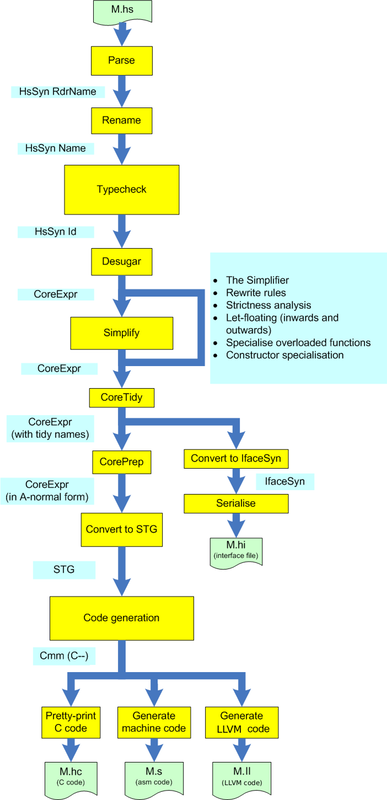
\includegraphics[width=0.7\textwidth]{images/AOSA_compiler}
    \caption[Schemat Glasgow Haskell Compiler]{Schemat Glasgow Haskell Compiler\cite{AOSA}}
    \label{fig:AOSA_compiler}
\end{figure}

\subsection{Parser}\label{sec:parser}
Parsowanie w~GHC dzieli się na etapy analizy leksykalnej i~składniowej. Jest to
proces tak dobrze opracowany od strony algorytmicznej, że istnieją narzędzia,
które pozwalają na generowanie gotowych lekserów i~parserów z~opisu gramatyki.

W~czasie analizy leksykalnej plik na wejściu jest skanowany, dzielony na ciągi
znaków, tzw. leksemy i~generowany jest z~niego strumień wartości zwanych tokenami.
W~GHC tokeny to wartości typu \code{Token}, zdefiniowanego w~pliku \code{Lexer.x}.
Gramatyka leksykalna składa się z~szeregu wyrażeń regularnych i~odpowiadających im tokenów.
Leksemy wyodrębniane są, gdy dojdzie do dopasowania ciągu znaków na wejściu do jednego z~wyrażeń.
Stosowana jest metoda najdłuższego dopasowania, to znaczy lekser
wczytuje kolejne znaki tak długo, dopóki przynajmniej jedno wyrażenie akceptuje
wczytany podciąg. Po dopasowaniu lekser zwraca token odpowiadający temu wyrażeniu.
Proces ten jest kontynuowany do przetworzenia całego wejścia.

W~GHC lekser jest generowany z~wykorzystaniem narzędzia Alex. Definicja
gramatyki leksykalnej zawarta jest w~pliku \code{Lexer.x}. W~przykładzie
\ref{lst:alex_example} pokazane są fragmenty tego pliku. Na początku widoczne są
makra, za którymi stoją wyrażenia regularne. Na końcu fragmentu pokazane jest
kilka reguł z~tymi makrami po lewej stronie i~wyrażeniami, które mają zostać
zwrócone po dopasowaniu do danego wyrażenia regularnego. Znajdujące się tam
\code{idtoken}, \code{varid} itd. to zwykłe funkcje w~Haskellu, zdefiniowane
w~innym miejscu, które zwracają tokeny\cite{DocsAlex}.

\begin{lstlisting}[float,label={lst:alex_example},
                   caption={Wycinki z pliku \code{Lexer.x} składające się na reguły opisujące co jest wyodrębniane jako zmienna i konstruktor.}]
$unilarge  = \x01 -- Trick Alex into handling Unicode. See alexGetByte.
$asclarge  = [A-Z]
$large     = [$asclarge $unilarge]

$unismall  = \x02 -- Trick Alex into handling Unicode. See alexGetByte.
$ascsmall  = [a-z]
$small     = [$ascsmall $unismall \_]

$ascdigit  = 0-9
$unidigit  = \x03 -- Trick Alex into handling Unicode. See alexGetByte.
$digit     = [$ascdigit $unidigit]

$digit     = [$ascdigit $unidigit]
$suffix    = \x07 -- Trick Alex into handling Unicode. See alexGetByte.
$idchar    = [$small $large $digit $suffix \']

@varid     = $small $idchar*          -- variable identifiers
@conid     = $large $idchar*          -- constructor identifiers

@qual = (@conid \.)+
@qvarid = @qual @varid
@qconid = @qual @conid

haskell :-
<0,option_prags> {
  @qvarid                       { idtoken qvarid }
  @qconid                       { idtoken qconid }
  @varid                        { varid }
  @conid                        { idtoken conid }
}
\end{lstlisting}

W~czasie analizy składniowej strumień tokenów zamieniany jest w~bardziej złożoną
strukturę, drzewo składniowe. W~GHC parser, tak jak lekser, został wygenerowany
automatycznie. Wykorzystano do tego narzędzie Happy. Definicja gramatyki w~formacie akceptowanym
przez Happy znajduje się w~pliku \code{Parser.y}. Jest podana w~notacji Backusa-Naura
wzbogaconej, podobnie jak w~Alex, o~fragmenty kodu w~Haskellu wywoływane w~celu
stworzenia struktury danych reprezentującej to drzewo\cite{DocsHappy}. Przykład
\ref{lst:happy_example} pokazuje wybrane produkcje z~tego pliku, wykorzystujące
przy tym token \code{ITvarid} zwracany przez funkcję \code{varid} z~przykładu
\ref{lst:alex_example}.

\begin{lstlisting}[float,label={lst:happy_example},
                   caption={Wycinki z pliku \code{Parser.y} z produkcjami odpowiadającymi za zmienne typów, wykorzystujące tokeny, których dotyczył przykład \ref{lst:alex_example}.}]
%token
 VARID          { L _ (ITvarid    _) }          -- identifiers
 CONID          { L _ (ITconid    _) }

tyvar   :: { Located RdrName }
tyvar   : tyvarid               { $1 }

tyvarid :: { Located RdrName }
        : VARID            { sL1 $1 $! mkUnqual tvName (getVARID $1) }
        | special_id       { sL1 $1 $! mkUnqual tvName (unLoc $1) }
        | 'unsafe'         { sL1 $1 $! mkUnqual tvName (fsLit "unsafe") }
        | 'safe'           { sL1 $1 $! mkUnqual tvName (fsLit "safe") }
        | 'interruptible'  { sL1 $1 $! mkUnqual tvName (fsLit "interruptible") }
\end{lstlisting}

\subsection{Renamer}\label{sec:renamer}

W~Haskellu, jak w~wielu innych językach, może istnieć kilka funkcji, zmiennych,
typów danych, klas, itd. o~tej samej nazwie. Na przykład, mogą one występować
w~różnych plikach albo w~lokalnym zakresie w konstrukcjach \code{let} lub
\code{where}. Z~tego powodu później ten sam identyfikator może odnosić się do
różnych rzeczy, w~zależności od tego, gdzie występuje i~co w~tym miejscu jest
widoczne w~zakresie. Kompilator, w~części zwanej renamerem, decyduje, do
której definicji odnosi się każde wystąpienie danej nazwy.

Każda osobna definicja otrzymuje na tym etapie unikalny, wewnętrzny identyfikator.
Następnie nazwy w~programie są zamieniane na odniesienia do jednej z~tych
zmiennych. Utrzymywany jest w~tym celu słownik nazw znajdujących się w~danej
chwili w~zakresie. Jeżeli w~danym miejscu nie da się na podstawie zawartości
słownika jednoznacznie określić, do czego odnosi się pewne wystąpienie nazwy, to
wywoływany jest błąd, jak w~przykładzie \ref{lst:renamer_ambiguous}. W~algorytmie
brane jest przy tym pod uwagę, czy nazwa jest kwalifikowana i~w~jaki sposób
importowany jest inny moduł, co czasami pozwala usunąć wieloznaczność. Możliwe jest również
zjawisko zwane \foreign{shadowingiem}, polegające na zastąpieniu umieszczonej w~zakresie
definicji przez definicję lokalną. Zachodzi ono na fragmencie
\ref{lst:renamer_shadowing}. Wreszcie, jeżeli w~danym miejscu w~zakresie nie
będzie nic o~danej nazwie, to renamer zakończy działanie z~błędem, jak
w~przykładzie \ref{lst:renamer_missing}.

\begin{lstlisting}[float,label={lst:renamer_ambiguous},
                   caption={Przykład działania renamera - niejednoznaczne odwołanie.}]
import Data.Maybe (isJust)

isJust :: Maybe a -> Bool
isJust Nothing = False
isJust _ = True

main :: IO ()
main = print $ isJust (Just 0)

{- Wywołuje błąd:
renamer.hs:8:16:
    Ambiguous occurrence ‘isJust’
    It could refer to either ‘Main.isJust’, defined at renamer.hs:4:1
                          or ‘Data.Maybe.isJust’,
                             imported from ‘Data.Maybe’ at renamer.hs:1:20-25
-}
\end{lstlisting}

\begin{lstlisting}[float,label={lst:renamer_shadowing},
                   caption={Przykład działania renamera - shadowing.}]
foo = 10

main :: IO ()
main = let foo = 20 in print foo

-- Po uruchomieniu wypisze 20
\end{lstlisting}

\begin{lstlisting}[float,label={lst:renamer_missing},
                   caption={Przykład działania renamera - nieodnalezienie w zakresie.}]
main :: IO ()
main = print bar

-- Wywołuje błąd:
-- renamer3.hs:2:14: Not in scope: ‘bar’
\end{lstlisting}

Na tym etapie kompilacji wykonywane jest również wiele pobocznych zadań, na
przykład wyświetlenie ostrzeżeń, gdy pewna zmienna zostanie zdefiniowana, lecz
nie będzie później użyta w~wyrażeniu, gdy kompilacja została rozpoczęta z~flagą
\code{-fwarn-unused-matches}. To zachowanie jest jednym z~usprawnień poruszonych w~tej pracy.

\subsection{Type checker}\label{sec:type_checker}

Warto w~tym miejscu wspomnieć o~podstawowych pojęciach związanych z~systemami
typów. Częścią definicji języka jest jego gramatyka, która określa, jakie ciągi
znaków można uznać za program w~tym języku. W~skład gramatyki wchodzą wyrażenia,
które w~wielu językach można podzielić na termy i~typy.

Termy pozwalają wyrażać obliczenia, dzięki zdefiniowanej dla nich semantyce.
Jednym z~rodzajów semantyki jest semantyka operacyjna, w~której wykonywanie
obliczeń modeluje się za pomocą maszyny stanowej. Term jest lub, w~bardziej
złożonych semantykach, zawiera się w~stanie maszyny. Ponadto istnieje relacja
przejścia, określającej stany do jakich przechodzi maszyna w~wyniku obliczeń.
Semantykę operacyjną określa się przez przez podanie reguł ewaluacji, z~których
wynika ta relacja.

Wykonywanie programu może zatrzymać się w~stanie uważanym za końcowy. Term
w~postaci, do której został znormalizowany w~stanie końcowym, nazywamy wartością.
Obliczenia mogą również nigdy nie zatrzymać lub utknąć w~stanie, który nie jest
końcowy, lecz dla którego relacja przejścia nie określa dalszych kroków.
Termy, dla których ewaluacja daje taki rezultat, nazywamy niepoprawnymi lub
bezsensownymi\cite{TAPL}. Przykład \ref{lst:types_nonsense} pokazuje niepoprawny term.

\begin{lstlisting}[float,label={lst:types_nonsense},
                   caption={Przykład bezsensownego wyrażenia w programie, z błędem GHC, który wywołuje.}]
module Nonsense where

nonsense = 10 + "a"

{- Błąd kompilacji w GHC:
[1 of 1] Compiling Nonsense         ( nonsense.hs, nonsense.o )

nonsense.hs:3:15:
    No instance for (Num [Char]) arising from a use of ‘+’
    In the expression: 10 + "a"
    In an equation for ‘nonsense’: nonsense = 10 + "a"
-}
\end{lstlisting}

Typy są przyporządkowywane termom w~relacji typowania, wynikającej z~pewnych
reguł typowania. Zbiór tych reguł składa się na system typów. System typów służy do
wykrywania bezsensownych termów bez ich ewaluowania, często już na etapie kompilacji.
System typów jest poprawny (\foreign{sound}) lub bezpieczny,
jeżeli każdy term, który ma w~nim przyporządkowany typ, jest sensowny. Z~kolei
jest zupełny (\foreign{complete}), jeżeli każdy sensowny term jest w~nim otypowany.
Systemy typów w~popularnych językach są przeważnie poprawne, lecz niezupełne. Rozszerzenia
systemu typów dążą do zmniejszenia liczby poprawnych programów, które są
w~systemie typów niedopuszczalne, co można określić jako zwiększenie jego
ekspresywności. Rozszerzenia mogą doprowadzić do tego, że problem sprawdzenia,
czy dany program jest poprawnie otypowany, stanie się nierozstrzygalny. Nie
będzie wtedy możliwe stworzenie odpowiedniego algorytmu i~zagwarantowanie, że
proces kompilacji się zakończy. Może to być niedopuszczalne ze względu na
oczekiwania użytkowników - programistów\cite{TAPL}.

\begin{lstlisting}[float,label={lst:types_diverge},
                   caption={Przykład programu, dla którego statyczne sprawdzanie typów w GHC się nie zakończy.}]
{-# LANGUAGE TypeFamilies, UndecidableInstances #-}

module Diverge where

type family Diverge a where
   Diverge a = Diverge a

evil :: Diverge Int
evil = 0
\end{lstlisting}

Polimorfizm to możliwość posiadania przez term więcej niż jednego przypisanego
mu typu. Może on wtedy występować w~miejscach, gdzie oczekiwany jest term jednego
z~tych typów.

W~polimorfizmie parametrycznym uzyskuje się to przez wprowadzenie
do typu zmiennych, za które mogą być podstawiane inne typy. Termy otypowane w~ten
sposób muszą mieć sens niezależnie od tego, jakie typy zostaną przyporządkowane
zmiennym, choć np. w~Haskellu istnieje możliwość wprowadzenia ograniczeń na zmienne.
Polimorfizm parametryczny odpowiada kwantyfikacji ogólnej z~logiki. Typy takie
mogą mieć składnię pozwalającą na zapisanie jawnego kwantyfikatora, wiążącego
zmienne w~typie, zamiast pozostawiania tych zmiennych jako niezwiązanych.
W~przykładzie \ref{lst:poly_parametric} funkcja \code{twice} jest polimorficzna,
w~jednym miejscu zmienna \code{a} służy za \code{Bool}, a~w~drugim za \code{String}.
Funkcja \code{twice'} pokazuje wspomnianą jawną kwantyfikację, lecz poza tym jest
równoważna poprzedniej funkcji. W~języku Java polimorfizm parametryczny
dostępny jest pod postacią typów generycznych.

\begin{lstlisting}[float,label={lst:poly_parametric},
                   caption={Przykład użycia polimorfizmu parametrycznego w Haskellu.}]
{-# LANGUAGE ExplicitForAll #-}

twice :: (a -> a) -> a -> a
twice f = f . f

twice' :: forall a . (a -> a) -> a -> a
twice' f = f . f

main :: IO ()
main = do
    print $ twice not True         -- True
    print $ twice ('-':) "Hello"   -- "--Hello"
\end{lstlisting}

W~polimorfizmie ad hoc term może mieć przypisane różne typy dzięki temu,
iż ma wiele definicji. W~zależności od typu wykorzystywana jest inna z~nich.
W~Haskellu ten polimorfizm jest dostępny w~postaci klas typów\cite{TAPL}.
W~przykładzie \ref{lst:poly_adhoc} funkcja \code{foo} występuje raz jako
funkcja typu \code{Bool -> Int} i~raz jako \code{String -> Int}. W~każdym
przypadku ma inną definicję, sensowną dla wybranego wtedy typu. W~Javie
polimorfizm ten występuje pod postacią przeładowania metod, jak w~przykładzie
\ref{lst:poly_adhoc_java} z~metodą \code{bar}.

\begin{lstlisting}[float,label={lst:poly_adhoc},
                   caption={Przykład użycia polimorfizmu ad hoc w Haskellu.}]
class C a where
    foo :: a -> Int

instance C Bool where
    foo True = 1
    foo _    = 0

instance C [a] where
    foo = length

main :: IO ()
main = do
    print $ foo True      -- 1
    print $ foo "Hello"   -- 5
\end{lstlisting}

\begin{lstlisting}[float,language=Java,label={lst:poly_adhoc_java},
                   caption={Przykład użycia polimorfizmu ad hoc w Javie.}]
public class Parametric {
    public static void main(String... args) {
        bar(10);       // bar int 10
        bar("str");    // bar String str
    }

    static void bar(int arg) {
        System.out.println("bar int " + arg);
    }

    static void bar(String arg) {
        System.out.println("bar String " + arg);
    }
}
\end{lstlisting}

W~kompilatorze sprawdzenie, czy program jest poprawnie otypowany, zachodzi w~części
zwanej type checkerem. Jednym z~zadań type checkera jest wyświetlenie w~razie błędu takich
komunikatów, by pozwolić użytkownikowi zrozumieć problem i~go naprawić.
Z~tego powodu aż do tego etapu kompilacji zachowywane są takie informacje
jak lokalizacja w~pliku wejściowym i~identyfikatory wybrane przez użytkownika.

\section{Rozszerzenia Glasgow Haskell Compiler}\label{sec:rozszerzenia_ghc}

Przez rozszerzenia GHC rozumiane są zaimplementowane w~nim funkcje, które nie są
częścią specyfikacji języka przedstawioną w~Haskell 2010 Language
Report. Zliczenie linii w~rezultacie wywołania \code{ghc --supported-extensions}
pozwala stwierdzić, że jest ich obecnie około stu. Rozszerzenia są opcjonalne
i~domyślnie wyłączone. Uaktywnia się je dyrektywą języka umieszczoną na początku
pliku modułu lub przez podanie odpowiednich flag wśród argumentów wywołania
kompilatora. Wszystkie zmiany wykonane w~tej pracy wiążą się z~pewnymi
rozszerzeniami, dlatego warto je omówić.

\subsectionex{Rodziny typów}{Rozszerzenie \code{TypeFamilies}}\label{sec:rodziny_typow}

Rodziny typów to funkcje operujące na typach w~trakcie kompilacji.
Stworzenie rodziny typów wymaga podania deklaracji rodziny z~liczbą i~rodzajami
parametrów oraz pewnej liczby definicji lub równań. W~przypadku rodzin związanych
z~klasą, deklaracja znajduje się w~deklaracji klasy i~musi wykorzystywać parametry
klasy. Przykładem takiej rodziny jest \code{Box} z~klasy \code{T} na
fragmencie \ref{lst:typefams_assoc_standalone}. Może dodatkowo
posiadać równanie domyślne, o~takim samym znaczeniu co domyślne definicje
funkcji w~klasie. Równania podaje się przy definiowaniu instancji klasy.
W~przypadku rodzin niezależnych od klasy, jak \code{Cont} z~przykładu
\ref{lst:typefams_assoc_standalone}, deklarację tworzy się z~użyciem słowa
kluczowego \code{family}, a~równania tworzy się ze słowem kluczowym \code{instance}.

\begin{lstlisting}[float,label={lst:typefams_assoc_standalone},
                   caption={Przykład pozwiązanej z klasą i niezależnej rodziny typów.}]
{-# LANGUAGE TypeFamilies #-}

module TypeFamilies where

class T a where
    data Box a
    store :: Box a -> a -> Box a

instance T Int where
    data Box Int = BoxI0 | BoxI1 Int
    store BoxI0 n = BoxI1 n
    store (BoxI1 acc) n = BoxI1 $ acc + n

instance T Bool where
    data Box Bool = BoxB0 Int Int
    store (BoxB0 ts fs) True = BoxB0 (ts + 1) fs
    store (BoxB0 ts fs) _    = BoxB0 ts (fs + 1)


data family Cont a
data instance Cont Int = ContI0 | ContI1 Int
data instance Cont Bool = ContB0 Int Int

class S a where
    put :: Cont a -> a -> Cont a

instance S Int where
    put ContI0 n = ContI1 n
    put (ContI1 acc) n = ContI1 $ acc + n

instance S Bool where
    put (ContB0 ts fs) True = ContB0 (ts + 1) fs
    put (ContB0 ts fs) _    = ContB0 ts (fs + 1)
\end{lstlisting}

Rodziny typów dzielą się na rodziny synonimów typów, deklarowane ze słowem
kluczowym \code{type} i~rodziny typów danych, deklarowane ze słowem
kluczowym \code{data}. Równania należące do rodzin synonimów tworzą synonimy typów,
podobne do tych z~nierozszerzonego Haskella. W~przykładzie \ref{lst:typefams_open_close}
\code{Equal Int Int} jest synonimem \code{Int} i~oba równie dobrze mogą znaleźć
się w~deklaracji typu dla \code{foo}. Analogicznie, rodziny typów danych grupują
typy danych \code{data} lub \code{newtype}. Na przykład \code{Cont Int} z~przykładu
\ref{lst:typefams_assoc_standalone} to nazwa typu danych, którego wartości konstruuje się
z~użyciem \code{ContI0} lub \code{ContI1}.

Rodziny synonimów mogą mieć postać otwartą i~zamkniętą. W~formie
zamkniętej, wszystkie równania rodziny wymienione są w~miejscu jej
deklaracji. Mają tę zaletę wobec rodzin otwartych, iż poszczególne równania mogą na
siebie nachodzić i~w~takim wypadku stosowany jest synonim, którego równanie jest
pierwsze od góry. Przypomina to mechanizm dopasowania wzorców dostępny na poziomie
termów. W~przypadku rodzin otwartych, kolejność równań nie jest
określona i~mogą one być definiowane w~wielu plikach, więc nachodzenie na siebie
dziedzin równań powoduje błąd. Różnicę tę widać w~przykładzie
\ref{lst:typefams_open_close}\cite{GuideTypeFamilies}.

\begin{lstlisting}[float,label={lst:typefams_open_close},
                   caption={Przykład otwartej i zamkniętej funkcji na typach z nachodzącymi na siebie dziedzinami.}]
{-# LANGUAGE TypeFamilies #-}

module TypeFamilies where

type family Equal a b where
    Equal a a = a
    Equal a b = (a, b)

foo :: Equal Int Int
foo = 10

type family Open a b
type instance Open a a = a
type instance Open a b = (a, b)

{-
families-overlapping.hs:13:15:
    Conflicting family instance declarations:
      Open a a -- Defined at families-overlapping.hs:13:15
      Open a b -- Defined at families-overlapping.hs:14:15
-}
\end{lstlisting}

\subsectionex{Częściowe sygnatury typów}{Rozszerzenie \code{PartialTypeSignatures}}\label{sec:partial_sigs}

W~Haskellu, podczas definiowania wyrażenia, możliwe, i~zgodne z~dobrymi
praktykami, jest podanie sygnatury typu. Jest to jednak opcjonalne, gdyż przy
braku sygnatury w~czasie sprawdzania typów dojdzie do próby
rekonstrukcji. Istnieje jednak również inna, pośrednia opcja: podanie niepełnej
sygnatury, zawierającej tak zwane symbole wieloznaczne, zapisywane w~postaci
podkreślnika.

Domyślnie obecność wieloznacznika wywoła błąd, w~którego treści znajdzie się
zrekonstruowany typ, którym można uzupełnić sygnaturę, a~kompilacja zostanie
przerwana. Rozszerzenie \code{PartialTypeSignatures} zmieni jednak to
zachowanie, sprawiając, iż zamiast błędu wygenerowane zostaną jedynie
ostrzeżenia i~obecność wieloznacznika nie będzie przyczyną zakończenia działania
kompilatora. Dodatkowo ostrzeżenia te można ukryć uruchamiając GHC z~flagą
\code{-fno-warn-partial-type-signatures}. Przykład
\ref{lst:partialsigs_infer_type} demonstruje przebieg kompilacji z~tym
rozszerzeniem.

\begin{lstlisting}[float,label={lst:partialsigs_infer_type},
                   caption={Przykład użycia anonimowego symbolu wieloznacznego w sygnaturze typu.}]
foo :: _ -> Bool
foo = not

{- Wywoła błąd lub ostrzeżenie:
partial.hs:3:8:
    Found hole ‘_’ with type: Bool
    To use the inferred type, enable PartialTypeSignatures
    In the type signature for ‘foo’: _ -> Bool
-}
\end{lstlisting}

Symbol wieloznaczny może także znaleźć się wśród ograniczeń klasowych jak
w~przykładzie \ref{lst:partialsigs_infer_constraints}. Wtedy w~błędzie lub
ostrzeżeniu, generowanym na takich samych zasadach, co w~poprzednim przypadku,
znajdą się wywnioskowane przez kompilator zero lub więcej ograniczeń. Oprócz
wieloznacznika w~sygnaturze mogą znaleźć się jawnie podane ograniczenia.

\begin{lstlisting}[float,label={lst:partialsigs_infer_constraints},
                   caption={Przykład użycia anonimowego symbolu wieloznacznego w ograniczeniach typu.}]
bar :: _ => [a] -> Bool
bar (x:y:_) = x == y
bar _ = False

{- Wywoła błąd lub ostrzeżenie:
partial-constr.hs:3:8:
    Found hole ‘_’ with inferred constraints: (Eq a)
    To use the inferred type, enable PartialTypeSignatures
    In the type signature for ‘bar’: _ => [a] -> Bool
-}
\end{lstlisting}

Drugim rozszerzeniem związanym z~częściowymi sygnaturami jest
\code{NamedWildCards}. Sprawia ono, iż identyfikatory zaczynające się od
podkreślnika są również traktowane jako wieloznaczniki i~są traktowane w~podobny
sposób do tego zaprezentowanego w~\ref{lst:partialsigs_infer_type}
i~\ref{lst:partialsigs_infer_constraints}. Bez niego wyłącznie same podkreślniki
są traktowane jako wieloznaczniki, a~identyfikatory zaczynające się od
podkreślników jako zwyczajne zmienne typów. Te opcjonalne aktywowane wieloznaczniki
określane są jako wieloznaczniki nazwane, a~te opisane poprzednio jako
wieloznaczniki anonimowe.

Warte uwagi jest, iż nazwane wieloznaczniki to nie zmienne typów. Pokazuje to
przykład \ref{lst:partialsigs_named_wcs}, gdzie po aktywowaniu rozszerzenia
\code{NamedWildCards} podana sygnatura jest poprawna, z~wywnioskowanym typem
\code{Bool} w~miejscu \code{\underscore x}. Bez tego rozszerzenia z~kolei jest
ona niepoprawna, gdyż \code{\underscore x} jest wtedy traktowana jako zwykła
zmienna, a~zatem \code{foo} jest wtedy funkcją polimorficzną, która powinna mieć
sens dla każdego \code{\underscore x}, co wyraźnie nie jest prawdą dla wyrażenia
\code{not \underscore x}\cite{GuidePartialTypeSignatures}.

\begin{lstlisting}[float,label={lst:partialsigs_named_wcs},
                   caption={Demonstracja różnicy między zmienną z podkreślnikiem i nazwanym wieloznacznikiem.}]
omodule Partial where
foo :: _x -> (Bool, _x)
foo a = (True, not a)

foo :: _ -> Bool
foo = not

{- Wywoła błąd lub ostrzeżenie:
partial-named.hs:4:16:
    Couldn't match expected type ‘_x’ with actual type ‘Bool’
      ‘_x’ is a rigid type variable bound by
           the type signature for foo :: _x -> (Bool, _x)
           at partial-named.hs:3:8
    Relevant bindings include
      a :: _x (bound at partial-named.hs:4:5)
      foo :: _x -> (Bool, _x) (bound at partial-named.hs:4:1)
    In the expression: not a
    In the expression: (True, not a)
-}
{- Z rozszerzeniem NamedWildCards:
partial-named.hs:3:8:
    Found hole ‘_x’ with type: Bool
    To use the inferred type, enable PartialTypeSignatures
    In the type signature for ‘foo’: _x -> (Bool, _x)
-}
\end{lstlisting}

\chapter{Użyte narzędzia i technologie}\label{chap:technologie}

\section{Zbiór danych}\label{sec:zbior_danych}

\subsection{RedDots}

W pracy wykorzystano zbiór \techname{RedDots}\cite{theReddotsDataCollection}.
Jest to zbiór nagrań głosowych przeznaczony do problemu weryfikacji mówcy.
Jest dostosowany do problemu weryfikacji zależnej od tekstu, gdyż transkrypcja każdej wypowiedzi jest znana,
a mówcy wypowiadają w nim wielokrotnie zdania o tej samej treści. Zbiór został zebrany od ochotników z całego
świata przez Internet, co sprawia, że choć treści wypowiedzi są po angielsku, to mówcy wypowiadają słowa
z różnym akcentem. Nagrania były tworzone w niekontrolowanych warunkach i często są zakłócone.
Wśród ochotników znalazło się 49 mężczyzn i 13 kobiet z 21 krajów.

Gromadzenie danych przebiegało w cotygodniowych sesjach. Autorzy mieli plan zebrać po 52 sesji od każdego uczestnika,
czyli zbierać je przez cały rok, ale w praktyce liczba sesji na mówcę jest bardzo różna. Łącznie przeprowadzono
473 sesji mężczyzn i 99 sesji kobiet, gromadząc 15306 nagrań. W każdej sesji uczestnik miał za zadanie nagrać 24 wypowiedzi.

\begin{itemize}
    \item 10 wypowiedzi miało stałą treść dla wszystkich uczestników i we wszystkich sesjach. Stanowią one podstawę
        pierwszego zadania testowego zdefiniowanego przez twórców. Ich treść to zdania o identyfikatorach $31-40$
        z innego zbioru \shortcut{TIMIT}.
    \item 10 wypowiedzi miało stałą treść we wszystkich sesjach, lecz unikalną dla każdego uczestnika. To znaczy
        każdemu uczestnikowi przydzielono na stałe oddzielny zestaw 10 zdań. Nagrania te są podstawą drugiego zadania.
    \item 2 wypowiedzi o treści nie zmieniającej się między sesjami, lecz wybranej przez uczestnika. Powoduje
        to w porównaniu z poprzednim punktem ryzyko, iż użytkownik wybierze krótkie hasło. Do tego niektórzy
        użytkownicy wybierali zdania w innym języki niż angielski. Pozwala to zbadać efekty pozostawienia wyboru hasła
        użytkownikom i jest przedmiotem trzeciego zadani.
    \item 2 wypowiedzi o treści unikalnej w całym zbiorze. Na ich treść składają się wycinki Wikipedii. Są wykorzystywane
        w czwartym zadaniu, które sprawdza skuteczność systemu na nagraniach o niezarejestrowanej wcześniej treści.
\end{itemize}

Wszystkie nagrania są w nieskompresowanym formacie \shortcut{pcm}, który oznacza, że wartości kolejnych próbek w czasie
są zapisane jedna po drugiej. Częstotliwość próbkowania nagrań to $16$kHz. Do tego zbiór zawiera plik z transkrypcjami
wszystkich wypowiedzi.

Poza tym są pliki z definicjami czterech problemów. Do każdego zadania zdefiniowany został zestaw nagrań rejestracyjnych
(\foreign{enrollment}) i zestaw nagrań weryfikacyjnych. (\foreign{trial}) Zadania te zostały wstępnie przedstawione
w opisie jakie 24 zdania wchodziły w skład sesji.

\begin{enumerate}
    \item Wszyscy mówcy wypowiadają te same 10 zdań. Trzy nagrania na zdanie na osobę przeznaczone są do zapisów. W testach
        są pozostałe nagrania. Każde jest wielokrotnie podawane do systemu w celu weryfikacji czy jest na nim oczekiwany mówca
        i zdanie. Dla każdego nagrania sprawdzane są wszystkie kombinacje znanych mówców i zdań z tej części. Do tego niektórzy
        mówcy nie są obecni w zbiorze rejestracyjnym i występują wyłącznie w zbiorze testowym. Stanowią oni test jak system
        radzi sobie przy otwartym zbiorze osób.
    \item Wszyscy mówcy wypowiadają po 10 zdań, każdy mówca ma swój unikalny zestaw. Podobnie jak powyżej, w zbiorze
        rejestracyjnym są po trzy nagrania na osobę na zdanie. Reszta nagrań służy do testów i niektórzy
        mówcy w testach nie występują w zbiorze rejestracyjnym.
        Jako że treść jest wyłączna dla użytkowników, to w przypadku, gdy mówca się nie zgadza, treść też się nie zgadza.
    \item Wszyscy mówcy wypowiadają po 2 zdania, każdy mówca ma unikalny zestaw. Mówcy sami decydują o treści.
        Przypadek podobny do poprzedniego, lecz wypowiedzi jest mniej i zdarzają się wypowiedzi w innych językach.
    \item
        \begin{enumerate}
            \item Wariant niezależny od tekstu. Zestaw rejestracyjny zawiera po sześć nagrań na osobę o unikalnej treści.
                Zestaw testowy zawiera nagrania, również o unikalnej treści.
            \item Wariant zależny od tekstu. Zestaw rejestracyjny zawiera nagrania z części 1-3. Zestaw testowy również
                zawiera nagrania z poprzednich części oraz dodatkowo nagrania z treścią unikalną w całym zbiorze.
        \end{enumerate}
\end{enumerate}

W przejrzanych pracach zwykle zadania 2 i 3 były ignorowane. Możliwe, że budzą mniejsze zainteresowanie przez fakt,
że różni mówcy zawsze różnią się treścią nagrania. Czyni to te części prostszymi, niż pozostałe dwie.
Dodatkowo nagrań w 3 części jest mniej.
Sprawdzenie jak system działa w sytuacji, gdy ktoś podszywa się pod mówcę i zna jego hasło jest bardzo
ważne w praktycznych zastosowaniach.  Do tego w niektórych pracach ignorowane
były nagrania kobiet, gdyż jest ich kilkakrotnie mniej niż nagrań mężczyzn.
Wszystkie testy uwzględniały część 1 i w większości uwzględniany był wariant części 4.

Zbiór został sporządzony na potrzeby konkursu w 2016 roku. Teraz jest dostępny za darmo pod warunkiem
ograniczenia wykorzystania do celów naukowych. Jest warty uwagi, gdyż trudno znaleźć
zbiór dostosowany do problemu weryfikacji zależnej od tekstu, który byłby publicznie dostępny i darmowy.
Istnieje na przykład zbiór \shortcut{YOHO} oraz zbiór \shortcut{RSR2015}, które
zawierają więcej danych zebranych w lepszych warunkach, lecz wymagają opłaty. Tym niemniej warto
o nich pamiętać.

\subsection{CMUDict}

\techname{CMUDict} to zbiór zawierający zapisy fonetyczne ponad 134000 angielskich słów. Rozróżnione
jest w nim 39 fonemów typowych dla angielskiego. Do tego w samogłoskach wyróżniony jest akcent.
Słowa mogą mieć więcej niż jeden zapis fonetyczny.

Zbiór został wykorzystany do zamiany transkrypcji z \techname{RedDots} na ciągi fonemów. Stała
za tym taka idea, że fonemy będą stanowić lepsze klasy w systemach rozpoznawania mówcy, jak
\shortcut{HMM-GMM}, niż litery, którym mogą w angielskim odpowiadać przeróżne fonemy.
Niestety niektóre wypowiedzi z części trzeciej, wybrane przez użytkowników, były w innych językach
i dla nich operacja zawiodła. Dlatego w systemach, które bazują na fonetycznych transkrypcjach,
są one odrzucane. Nie jest to problemem jeżeli zupełnie zignoruje się trzeci problem.

\section{Sprzęt}\label{sec:sprzet}

Utworzone w ramach pracy programy tworzono i wykonywano na maszynie udostępnionej
w Centrum Technologii Informatycznych Politechniki Łódzkiej. $64$GB pamięci i $40$ rdzeniowy
procesor mocno przyśpieszył pracę oraz umożliwił załadowanie całego zbioru do pamięci.
Praca nie wymaga jednak żadnych niestandardowych urządzeń lub warunków, jej odtworzenie
jest możliwe na zwykłym komputerze.

\section{Technologie}\label{sec:technologie}

\subsection{Język programowania}

Programy utworzone na potrzeby pracy stworzono w języku \techname{Python}. Wybrano go
ze względu na to, iż zdominował popularnością inne języki w dziedzinie przetwarzanie danych.
Wiąże się to z tym, iż istnieje dużo dojrzałych bibliotek, takich jak \techname{scikit-learn}
oraz \techname{TensorFlow}, zawierających implementacje metod, których wykorzystanie jest w planach.
Poza tym bezproblemowo integruje się środowiskiem \techname{Jupyter}, które jest bardzo wygodne przy
zdalnej pracy na klastrze. Umożliwia ono pracę interaktywną, co jest cenne, gdy zachodzi
potrzeba przetestowania wielu rozwiązań i reagowania na wyniki.

\subsection{Biblioteki}

\begin{figure}[H]
    \centering
    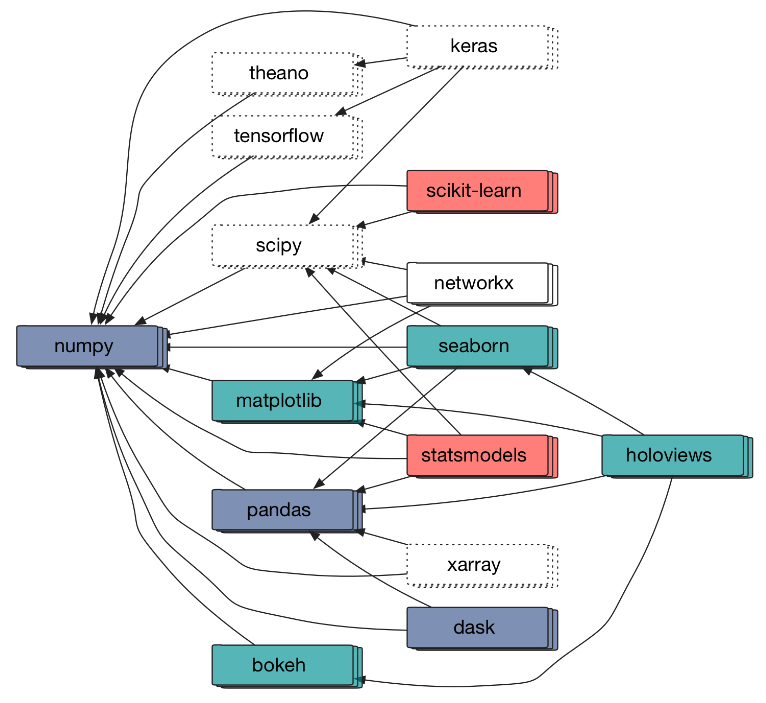
\includegraphics[width=0.6\textwidth]{images/3_3_ecosystem}
    \caption{Ekosystem narzędzi Pythonowych przedstawiony na prezentacji z PyData Warsaw 2017\cite{thePythonEcosystem}}
    \label{fig:3_3_ecosystem}
\end{figure}

Program wykorzystuje popularny \foreign{stack} związany z językiem \techname{Python} składający się z:

\begin{itemize}
    \item \techname{numpy} dostarczający wydajną i uniwersalną implementację macierzy wielowymiarowej i operacji na niej.
        Inne pakiety zależą od tej biblioteki i wykorzystują macierze w swojej implementacji.
    \item \techname{pandas} przede wszystkim udostępnia \foreign{DataFrame}, to znaczy obiekt do przechowywania i analizowania danych tabelarycznych, przypominający w funkcji arkusz kalkulacyjny. W porównaniu z macierzami z \techname{numpy}, \foreign{DataFrame} mogą składać się z kolumn różnych typów i o różnej semantyce. Przy operowaniu na nich często zachodzi potrzeba selekcji, grupowania bądź agregowania, liczenia statystyk opisowych wybranych kolumn.
    \item \techname{scipy} operuje na macierzach \techname{numpy} i dostarcza wiele algorytmów numerycznych, optymalizacyjnych, z algebry liniowej, statystycznych, itd. W tej pracy wykorzystano przede wszystkich moduł z metodami przetwarzania sygnałów.
    \item \techname{scikit-learn} zawiera algorytmy uczenia maszynowego. W pracy przydatna była przede wszystkim implementacja mikstur gaussowskich oraz obliczenia krzywej \shortcut{ROC}.
    \item \techname{matplotlib} pozwala na generowanie statycznych wizualizacji np. spektrogramów, krzywych \shortcut{ROC}. Z jej pomocą wygenerowane zostały także ilustracje konceptów z teorii przetwarzania mowy zaprezentowane w rozdziale \ref{chap:teoria}. Warto wspomnieć, że niektóre z tych ilustracji zostały wygenerowane z użyciem \techname{bokeh} i \techname{holoviews}.
    \item \techname{pickle} uniwersalna biblioteka do serializacji danych. Wykorzystana do zachowania dopasowanych modeli i wyników.
\end{itemize}

Jeśli chodzi o przetwarzanie dźwięku, to wykorzystany został pakiet \techname{python-speech-features}
do obliczenia \shortcut{MFCC} oraz cech delta i delta delta dla nagrań ze zbioru \techname{RedDots}.
Przed przetworzeniem cech używany jest również pakiet \techname{webrtcvad} do przeprowadzenia
\foreign{voice activity detection}, tzn. wykrycia ramek o niskiej energii.  Znalezione ramki z początku i końca są usuwane.

Przy pracach nad ukrytymi modelami Markowa wypróbowane zostały pakiety \techname{hmmlearn} i \techname{pomegranate}.
Niestety sprawiały wiele problemów numerycznych podczas dopasowywania modelu do nagrań. Ostatecznie zrezygnowano z nic
i zastąpiono własną implementacją.

W pracy użyty został również \techname{TensorFlow}. Biblioteka ta dostarcza
implementacji tensora - pozornie macierzy wielowymiarowej jak z \techname{numpy}. Jest jednak
dostosowana do potrzeb implementacji algorytmów uczenia maszynowego. Stosuje model opóźnionej
ewaluacji, podobnie jak \techname{Spark} lub \techname{dask}. To znaczy, że
osobno definiuje się w niej operacje do wykonanie przez zbudowanie grafu i osobno przekazuje go do interpretacji.
Ten sposób wykonania umożliwia dokonanie optymalizacji po zdefiniowaniu obliczeń i przed wykonaniem oraz
obchodzi się tym samym wadę Pythona - relatywnie powolne wykonywanie kodu.
\techname{Tensorflow} zawiera komponenty potrzebne do zdefiniowania grafu, w tym wysokopoziomowe
z pakietu \techname{tf.estimator}. Umożliwia automatyczne obliczanie pochodnych na potrzeby wstecznej propagacji.
Pozwala na wykonywanie operacji na \shortcut{GPU} oraz rozproszenie obliczeń.

W pracy użycie \techname{TensorFlowa} jest jednak ograniczone, gdyż w jej ramach nie jest trenowana żadna
sieć neuronowa. Wykorzystany został gotowy model stworzony przez organizację \techname{Mozilla} w oparciu o
pracę \techname{DeepSpeech}\cite{deepSpeechScaling}, opisującą komercyjny model do rozpoznawania mowy stworzony
przez \techname{Baidu}. Ten model jest wczytywany w sesji \techname{TensorFlowa} i używany do dopasowania
ramek do klas.

\subsection{Narzędzia}

W pracy wykorzystany został \techname{Docker}. Uruchamiany jest w nim obraz \techname{tensorflow/tensorflow:1.4.0-gpu-py3},
z przygotowanym środowiskiem z \techname{TensorFlowem}. Umożliwia to szybką instalację tego pakietu, która ogólnie nie
jest trywialna. W kontenerze uruchamiany jest serwer \techname{Jupyter} i z jego wykorzystaniem przebiegła większość prac.

\techname{Jupyter} stanowi rozwinięcie starszych narzędzi programowania interaktywnego jak \techname{IPython} czy zwykły \techname{Pythonowy} interpreter. W sesjach interaktywnych występuje taki problem, że instrukcje trzeba wprowadzać linijka po linijce, a wpisany kod jest zapisywany w ograniczonej historii. Przeciwieństwem sesji są skrypty, które pozwalają wygodnie manipulować
kodem oraz są trwałe i powtarzalne, lecz zupełnie nieinteraktywne i po każdej zmianie wymagają ponownego wykonania.
\techname{Jupyter} łączy dobre strony obu podejść i pozwala tworzyć skrypty, które można blokami wykonywać
w interaktywnej sesji, tzw. notesy. (\foreign{notebook}, format \techname{ipynb})

\techname{Jupyter} działa jako serwer \shortcut{HTTP} i dostarcza przeglądarkowe środowisko do edycji kodu. Jest ono
ubogie w funkcje, przynajmniej w porównaniu z rozwiniętymi środowiskami programistycznymi. Fakt, że
program działa jako serwer ma taką zaletę, iż można go uruchomić zdalnie na komputerze dysponującym duże zasoby
obliczeniowe oraz bezpośredni dostęp do danych, a następnie pracować na nim zdalnie.

Dużym atutem jest wsparcie dla bibliotek jak \techname{pandas}, \techname{matplotlib} czy \techname{bokeh}.
\foreign{DataFrame} są automatycznie wyświetlane jako tabele, a generowane wizualizacje są bezpośrednio wyświetlane
między blokami notesu. Jest też możliwość tworzenia interaktywnych elementów jak przyciski czy pola tekstowe i
w reakcji na zmiany ich stanu wykonywać kod w interaktywnej sesji.

Poza tym warto wspomnieć, że wykorzystano \techname{gita} do wersjonowania pracy, zarówno \foreign{notebooków}, pakietów jak i tekstu tego dokumentu. Do zarządzania pakietów wykorzystano \techname{pip}, ale być może lepszym wyborem są nowsze narzędzia jak \techname{conda} lub \techname{pipenv}.


\chapter{Stworzony system weryfikacji mówcy}\label{chap:badania}

\section{Przetworzenie danych}
\label{sec:data_wrangling}

Nagrania \techname{RedDots} zostały przetworzone w ten sposób:

\begin{itemize}
    \item Przeprowadzana jest procedura \shortcut{VAD} (\foreign{voice activity detection}), czyli wyodrębnianie
        fragmentów nagrania zawierających sygnał mowy, za pomocą pakietu \techname{webrtcvad}. Użyty parametr
        agresji $2$. Z każdego nagrania zostały usunięte ramki bezpośrednio z początku i z końca, które zostały
        uznane za ciche.
    \item Dla każdego obciętego nagrania obliczone zostały \shortcut{MFCC} korzystając z metody z
        pakietu \techname{python-speech-features}. Analizę przeprowadzono w oknach $25$ms z $10$ms skokiem.
        Użyto okna Hamminga. Utworzono $26$ filtrów pokrywających częstotliwości nagrania i zachowano z nich
        $13$. Użyto filtru \foreign{preemphasis} z parametrem $0.97$. Wynikiem jest $13$ współczynników.
    \item Dla każdej ramki obliczono cechy delta i delta-delta z użyciem pakietu \techname{python-speech-features}.
        Cechy te obliczono biorąc pod uwagę sąsiedztwo $4$ ramek przed i $4$ ramek po danej ramce.
    \item Bardzo krótkie nagrania, składające się z mniej niż $85$ ramek, zostały odrzucone. Kilka nagrań miało
        nawet długość $1$ ramki. Próg został wyznaczony przez zbadanie jakiej długości są nagrania. Między $85$
        i krótszymi jest skok, więc uznano je za anomalie.
\end{itemize}

Wykorzystano słownik \techname{CMUDict} do zamiany wszystkich transkrypcji z \techname{RedDots} na listy 39 fonemów
używanych w języku angielskim. Zignorowano przy tym akcenty. Części nagrań nie udało się zamienić, gdyż
zawierały treść w innym języku, i one nie będą używane w modelach wykorzystujących fonemy.

\section{Wykorzystane modele}
\label{sec:data_models}

W ramach pracy utworzone zostały trzy modele do weryfikacji mówcy. Zostały one tutaj opisane.

\subsectionex{Model GMM-UBM}{Mikstury gaussowskie z uniwersalnym modelem tła}
\label{sec:gmm_ubm}

System \shortcut{GMM-UBM} jest wzorowany na tym opisanym w pracy \cite{utteranceVerificationFor}. Posłużono
się również parametrami z tej pracy.

Wpierw zebrano wszystkie dane ze zbioru \techname{RedDots}, które nie są użyte w żadnym teście. Dopasowano
do nich model tła, który jest miksturą 512 dystrybucji normalnych. Założono, że cechy są nieskorelowane
i macierz kowariancji w miksturach jest diagonalna.

W ramach zapisów model tła jest kopiowany i \shortcut{MAP}-adaptowany z \foreign{relevance factor} równym $3.0$
dla nagrań rejestracyjnych danego mówcy. Dodatkowo dla każdej grupy nagrań o tej samej treści również tworzona
jest kopia modelu tła i \shortcut{MAP} adaptowana w ten sam sposób do nagrań z tej grupy.

W czasie testów dla każdego nagrania liczone jest prawdopodobieństwo, że nagranie pochodzi z modelu tła,
z \shortcut{GMM} mówcy, który jest oczekiwany w weryfikacji i z \shortcut{GMM} zdania, które jest oczekiwane.
Na podstawie tych wartości liczone są prawdopodobieństwa, że mówca i treść są poprawne jako stosunek prawdopodobieństw.

$$S_{sp}(x) = \frac{P(\theta_{sp} | x)}{max(P(\theta_{sp} | x), P(\theta_{UBM} | x))}$$
$$S_{st}(x) = \frac{P(\theta_{st} | x)}{max(P(\theta_{st} | x), P(\theta_{UBM} | x))}$$
$$S_{both}(x) = S_{sp}(x) S_{st}(x)$$

\subsectionex{Model HMM-GMM}{Ukryty model Markowa z emisjami w postaci mikstur gaussowskich}
\label{sec:hmm_gmm}

Ten model jest wzorowany na modelu opisanym w pracy \cite{comparisonOfMultiple}. Wykorzystuje
system rozpoznawania mowy do określenia, które ramki zawierają które fonemy. System ten
to ukryty łańcuch Markowa, w który każdy fonem jest reprezentowany przez trzy stany. Został
użyty model monofonemowy. Dla wypowiedzi w zbiorze znany jest ciąg fonemów, gdyż
\techname{RedDots} zawiera transkrypcje, które następnie zostały zamienione na fonemy
przez odszukanie odpowiednich słów w słowniku \techname{CMUDict}. Dla każdej wypowiedzi
budowany jest \shortcut{HMM} przez złączenie odpowiednich trójek stanów zgodnie z kolejnością
fonemów w wypowiedzi. Tworzony jest łańcuch z przejściami typu \foreign{beads-on-string}.

Dla każdego mówcy i tła budowany jest zestaw mieszanin \shortcut{GMM}, po jednej na stan \shortcut{HMM},
a zatem po trzy na fonem. Każda mikstura składa się z $8$ dystrybucji z diagonalną macierzą kowariancji.

Parametry podsystemu rozpoznawania mowy są wyznaczane tak, że najpierw do wszystkich danych
dopasowywana jest mała 8 składnikowa mikstura tła. Następnie budowane są wszystkie trójki \shortcut{GMM}
odpowiadające fonemom. Potem dla każdej wypowiedzi budowany jest model Markowa przez połączenie odpowiednich
trójek zgodnie ze znanym ciągiem fonemów danej wypowiedzi. Korzystając z \shortcut{HMM} i algorytmu Viterbiego
ramki nagrania są przyporządkowywane do części fonemów. Algorytm jest zmodyfikowany, by dawał wyższe prawdopodobieństwo
podziałowi, w którym każdemu ukrytemu stanowi odpowiada ta sama liczba ramek. To samo jest robione dla innych nagrań.
Następnie parametry trójek \shortcut{GMM} są dopasowywane przez \shortcut{EM} do ramek, które zostały im przypisane.
Po ustaleniu parametrów mikstur, ramki są przypisywane ponownie z użyciem algorytmu Viterbiego i proces jest ponawiany.

Rejestracje wyglądają tak, że dla każdego mówcy jest budowany jego zestaw trójek \shortcut{GMM}.
Wypowiedzi rejestracyjne danego mówcy są przyporządkowywane
częściom fonemów z użyciem algorytmu Viterbiego przez opisane \shortcut{HMM}.
Używając tego przyporządkowania mikstury tła są \shortcut{MAP} adaptowane do nagrań danego mówcy.

Testy wyglądają podobnie. Najpierw z użyciem systemu rozpoznawania mowy i algorytmu Viterbiego znajdowane
jest, które ramki zawierają które części fonemów. Następnie dla każdej ramki obliczany jest logarytm prawdopodobieństwa,
iż pochodzi ona z odpowiedniej mikstury mówcy i odpowiedniej mikstury tła. Sumując je uzyskiwany jest wynik dla mikstur
mówcy i mikstur tła. Wynik weryfikacji mówcy obliczany jest jako stosunek tych prawdopodobieństw. Treść
nagrania nie jest osobno sprawdzana.

$$S_{sp}(x) = exp(\sum_{x_i \in x} (log P(\theta_{sp} | x_i) - max(log P(\theta_{sp} | x_i), log P(\theta_{UBM} | x_i))))$$

\subsectionex{Model DNN-GMM}{Głęboka sieć neuronowa do dopasowania ramek, ocena miksturami gaussowskimi}
\label{sec:dnn_gmm}

W tym modelu wykorzystano głęboką sieć neuronową do rozpoznawania tekstu taką jak opisano w pracy \cite{endToEnd}.
Sieć składa się z pięciu warstw, w tym jednej rekurencyjnej warstwy \shortcut{LSTM}.
Wytrenowanie tej sieci wymaga niestety ogromnej ilości danych i czasu. Z raportów innych osób wynikało, że na
zwykłym komputerze pojedyncza epoka nauki może zająć nawet dwa tygodnie. Z tego powodu wykorzystany został
gotowy model stworzony przez organizację \techname{Mozilla}.

Model ten został wytrenowany na ok. 2500 godzinach nagrań ze zbiorów \techname{WSJ}, \techname{Switchboard}
i \techname{Fisher}. Warto zauważyć, że autorzy cytowanej pracy z \techname{Baidu} poza tymi zbiorami użyli
dodatkowo własnego, zamkniętego zbioru 5000 godzin nagrań. Sieć ta przyjmuje kolejne ramki, przy czym muszą
one być wstępnie przetworzone do współczynników \shortcut{MFCC}. Dla każdej chwili zwracany jest wektor 28 liczb,
które odpowiadają 25 literom alfabetu, przerwie, apostrofowi i szumowi.

Podobnie jak w \shortcut{HMM-GMM} dla każdego nagrania znamy treść i z wykorzystaniem systemu rozpoznawania
mowy przyporządkowujemy ramki literom. Istotna różnica jest taka, że tutaj system rozpoznawania mowy zwraca
tekst, nie sekwencje fonemów, co dla naszych potrzeb jest niepożądane. Gdyby trenować model od podstaw na
potrzeby rozpoznawania mówcy warto byłoby zmienić ten aspekt. Do przypisania ramek wykorzystano odpowiednio
dostosowany algorytm Viterbiego. Wyjścia sieci są w nim znormalizowane do przedziału $[0.0, 1.0]$ i traktowane
jako prawdopodobieństwa emisji danej ramki w kolejnych stanach ukrytych. Stany ukryte są tożsame z literami
i algorytm wymusza, by zmieniały się zgodnie ze znaną treścią oraz by wszystkie litery się pojawiły.
W przypadku, gdy największe prawdopodobieństwo przypada na szum algorytm pomija ramkę. Wynikiem
jest przypisanie do niektórych ramek liter oraz zwrócenie prawdopodobieństwa danej sekwencji - jak jest
bardzo małe to prawdopodobnie spodziewana treść i treść na nagraniu się różnią.

Trening wygląda analogicznie jak opisano w \shortcut{HMM-GMM}. To znaczy korzystając z przypisania ramek
zwróconego przez \shortcut{DNN}, tworzy się szereg \shortcut{GMM} z $8$ składnikami mikstury
i macierzami diagonalnymi, po jednym na literę. Następnie wyznaczane są ich parametry, by
maksymalizowały prawdopodobieństwo wystąpienia
ramek z ich klasy. Rejestracja wygląda tak samo, tylko \shortcut{MAP} adaptuje modele tła do
mniejszej liczby nagrań rejestracyjnych mówcy.

Metoda testowania ponownie polega na policzeniu stosunku prawdopodobieństw między \shortcut{GMM} mówcy, a tła.
Wynik jest sumowany dla wszystkich ramek, które mają przypisane litery. Weryfikacja treści nagrania
bazuje na prawdopodobieństwie zwróconym przez algorytm Viterbiego, czyli prawdopodobieństwie najbardziej
prawdopodobnej sekwencji przyporządkowań liter do ramek, w której litery zgadzają się z transkrypcją.

\section{Wyniki testów}
\label{sec:test_results}

W celu oceny systemów wykonano pierwsze zadanie zdefiniowane w zbiorze \techname{RedDots}. Każdy z modeli został
wykorzystany do zapisów mówców, a następnie do testów. Algorytm wykorzystania modeli wraz ze wszystkimi parametrami
zapisany jest w plikach \techname{Jupyter}, co powinno uczynić wyniki łatwymi do odtworzenia,
choć powtórzenie obliczeń może zająć dużo czasu.
Wyniki w postaci krzywej \shortcut{ROC}, \shortcut{EER} i \shortcut{AUC} zapisano w poniższej tabeli
i zwizualizowano pod tabelą.

\begin{table}[H]
    \centering
    \caption{Wyniki \shortcut{EER} i \shortcut{AUC} uzyskane przez modele \shortcut{GMM-UBM}, \shortcut{HMM-GMM}, \shortcut{DNN-GMM} na pierwszym zadaniu zdefiniowanym w zbiorze \techname{RedDots}}
    \label{tab:all_results}
    \small
    \tabulinesep =_3pt^3pt
    \begin{tabu}{l*{6}{r}}
        \multirow{2}{*}{Model} & \multicolumn{2}{c}{Tylko mówca} & \multicolumn{2}{c}{Tylko treść} & \multicolumn{2}{c}{Mówca i treść}
        \\
        & \shortcut{EER} & \shortcut{AUC} & \shortcut{EER} & \shortcut{AUC} & \shortcut{EER} & \shortcut{AUC}
        \\ \midrule
        \shortcut{GMM-UBM} & 4.69\% & 97.56\% & 6.04\% & 97.82\% & 3.20\% & 99.04\%
        \\
        \shortcut{HMM-GMM} & 15.86\% & 92.73\% & - & - & 5.16\% & 98.32\%
        \\
        \shortcut{DNN-GMM} & 39.51\% & 65.12\% & 17.65\% & 86.73\% & 24.24\% & 84.38\%
        \\
    \end{tabu}
\end{table}

\begin{figure}[H]
    \centering
    \begin{minipage}{.5\textwidth}
        \centering
        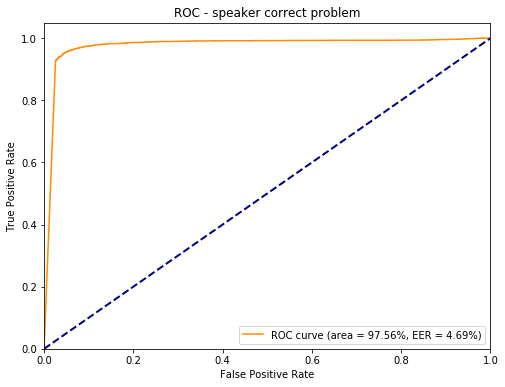
\includegraphics[width=0.8\textwidth]{images/4_3_gmm_roc_speaker}
        \label{fig:4_3_gmm_roc_speaker}
    \end{minipage}%
    \begin{minipage}{.5\textwidth}
        \centering
        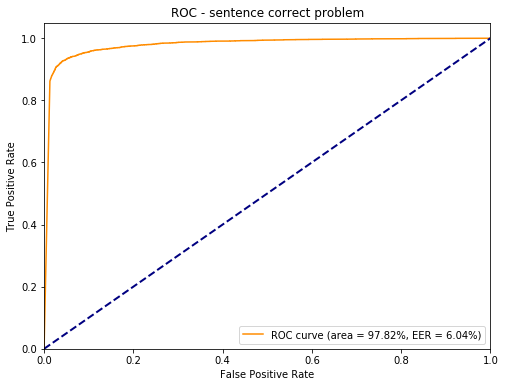
\includegraphics[width=0.8\textwidth]{images/4_3_gmm_roc_sentence}
        \label{fig:4_3_gmm_roc_sentence}
    \end{minipage}
    \caption{Wykresy krzywej \shortcut{ROC} dla \shortcut{GMM-UBM}, pierwszego zadania \techname{RedDots} i przypadków weryfikacji mówcy oraz weryfikacji treści}
\end{figure}

\begin{figure}[H]
    \centering
    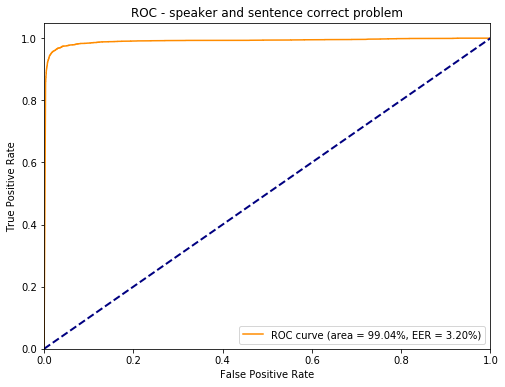
\includegraphics[width=0.6\textwidth]{images/4_3_gmm_roc_both}
    \caption{Wykres krzywej \shortcut{ROC} dla \shortcut{GMM-UBM}, pierwszego zadania \techname{RedDots} i jednoczesnej weryfikacji mówcy i treści}
    \label{fig:4_3_gmm_roc_both}
\end{figure}

\begin{figure}[H]
    \centering
    \begin{minipage}{.5\textwidth}
        \centering
        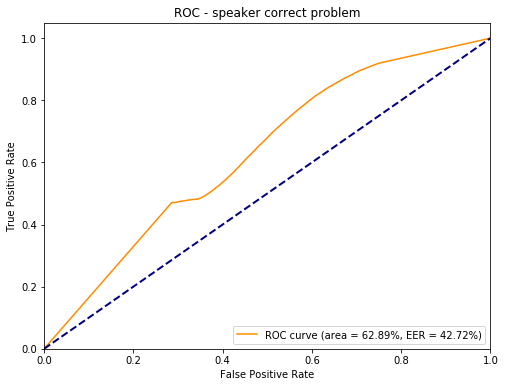
\includegraphics[width=0.9\textwidth]{images/4_3_dnn_roc_speaker}
        \label{fig:4_3_dnn_roc_speaker}
    \end{minipage}%
    \begin{minipage}{.5\textwidth}
        \centering
        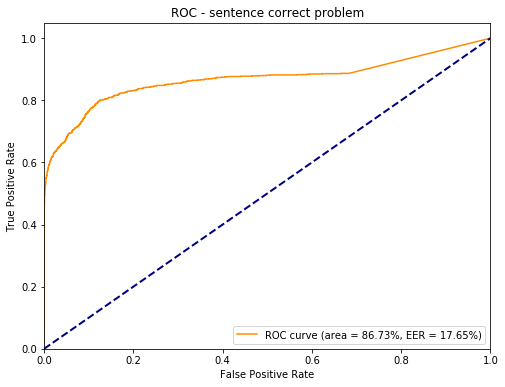
\includegraphics[width=0.9\textwidth]{images/4_3_dnn_roc_sentence}
        \label{fig:4_3_dnn_roc_sentence}
    \end{minipage}%
    \caption{Wykres krzywej \shortcut{ROC} dla \shortcut{DNN-GMM}, pierwszego zadania \techname{RedDots} i przypadków weryfikacji mówcy oraz weryfikacji treści}
\end{figure}

\begin{figure}[H]
    \centering
    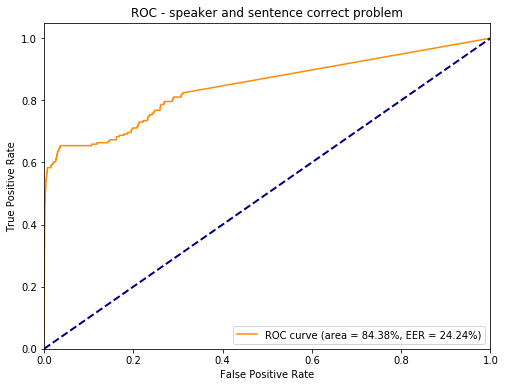
\includegraphics[width=0.6\textwidth]{images/4_3_dnn_roc_both}
    \caption{Wykres krzywej \shortcut{ROC} dla \shortcut{DNN-GMM}, pierwszego zadania \techname{RedDots} i jednoczesnej weryfikacji mówcy i treści}
    \label{fig:4_3_dnn_roc_both}
\end{figure}

\begin{figure}[H]
    \centering
    \begin{minipage}{.5\textwidth}
        \centering
        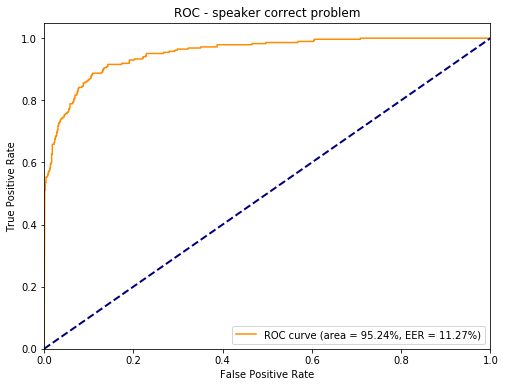
\includegraphics[width=0.9\textwidth]{images/4_3_hmm_roc_speaker}
        \label{fig:4_3_hmm_roc_speaker}
    \end{minipage}%
    \begin{minipage}{.5\textwidth}
        \centering
        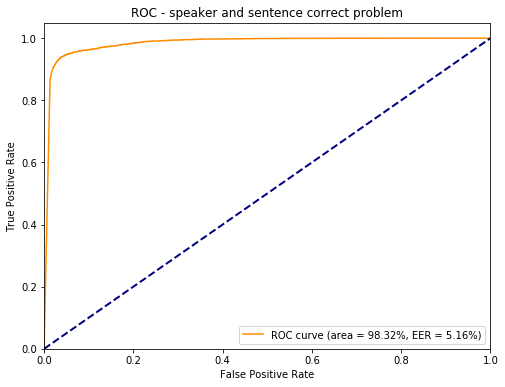
\includegraphics[width=0.9\textwidth]{images/4_3_hmm_roc_both}
        \label{fig:4_3_hmm_roc_both}
    \end{minipage}
    \caption{Wykres krzywej \shortcut{ROC} dla \shortcut{HMM-GMM}, pierwszego zadania \techname{RedDots} i przypadków weryfikacji mówcy oraz jednoczesnej weryfikacji mówcy i treści}
\end{figure}


\chapter{Podsumowanie i~wnioski}\label{chap:podsumowanie}

\section{Dyskusja wyników}

Dzięki zrealizowaniu pracy, sposób wyświetlania rodzin typów w~błędach
i~ostrzeżeniach kompilatora jest ujednolicony. Dodane zostało wyświetlanie prawych
stron równań rodzin typów danych w~sposób naśladujący składnię tych
konstrukcji. Stary sposób wyświetlania, oddający wewnętrzną reprezentację
rodzin typów danych, został zachowany w~zrzucie z~etapu sprawdzania typów.

Dodane zostało także opcjonalne wyświetlanie ostrzeżeń o~nieużywanych zmiennych
w~rodzinach typów. Zmienna uważana jest za nieużywaną jeżeli występuje we
wzorcach po lewej stronie równania tylko raz i~nie występuje w~typie po prawej
stronie.

Poprawiony został błąd z~zamianą zmiennych typów zaczynających się od
podkreślnika w~symbole wieloznaczne w~kontekstach, gdzie są one
niedozwolone. Algorytm renamera został również zmieniony tak, by nie dokonywał
zamiany zmiennych jawnie związanych kwantyfikatorem. Dzięki temu uaktywnienie
rozszerzenia \code{NamedWildCards} nie powoduje już odrzucania poprawnych programów.

Wszystkie te trzy modyfikacje przeszły proces rewizji kodu w~systemie
Phabricator i~znalazły się w~repozytorium. Od tamtej pory wprowadzony kod
podlegał dodatkowym modyfikacjom i~refaktoryzacji dokonanej przez innych
programistów. W~szczególności część dotycząca \code{NamedWildCards} została
w~dużej części zastąpiona przez alternatywne rozwiązanie Simona
Peytona Jonesa. Z~kolei ostrzeżenia o~nieużywanych zmiennych typów w~wyniku
zgłoszenia nr 11451 są uaktywniane nową flagą \code{-Wunused-type-variables}
zamiast \code{-Wunused-matches}.
Jednak wszystkie wprowadzone w tej pracy usprawnienia dalej są dostępne
w~kompilatorze, dlatego cele należy uznać za zrealizowane.

\section{Perspektywy dalszych badań}
System Trac na stronie GHC zawiera obecnie ponad 1600 otwartych
zgłoszeń\cite{WikiTickets}. W~innych pracach można podjąć się dokonania następnych
usprawnień związanych z~programowaniem z~użyciem typów lub z~inną częścią
kompilatora. Złożone propozycje mają poświęcone sobie podstrony na wiki GHC,
gdzie można znaleźć ich planowane funkcje, projekty, opisy przebiegu
implementacji i~odnośniki do prac badawczych, na których bazują. Są to na
przykład propozycja dodania typów zależnych do Haskella lub wprowadzenia
definiowanych przez użytkownika błędów typów. Praca mogłaby polegać również na
sformułowaniu nowej propozycji i~zaimplementowaniu jej. Możliwości są szerokie
i~wiele osób zdecydowało się już poświęcić swój czas GHC.


\bibliographystyle{plplain}
\bibliography{bibliografia}

\listoffigures
%\listoftables
\cleardoublepage
\addcontentsline{toc}{chapter}{\lstlistlistingname}
\lstlistoflistings

\appendix
\renewcommand{\chaptermark}[1]{%
\markboth{\MakeUppercase{%
DODATEK \thechapter.%
\ }}{}}
\chapter{Płyta CD}\label{app:plyta}

\begin{figure}[htb]
\makebox[\textwidth]{\framebox[12.8cm]{\rule{0pt}{12.8cm}}}
\end{figure}
\pagebreak

Zawartość katalogów na płycie:
\begin{description}
    \item[doc] : elektroniczna wersja pracy dyplomowej oraz dwie prezentacje wygłoszone podczas seminarium dyplomowego
    \item[src] : repozytorium z kodem źródłowym aplikacji
%    \item[web] : kopie źródeł elektronicznych umieszczonych w bibliografii
\end{description}

Miejsce budowania modeli i wizualizacje zawarte są w katalogu \textbf{src/notebooks} w postaci notatników \foreign{Jupyter}. Są to pliki z rozszerzeniem \textbf{.ipynb}. Wykonanie ich wymaga uruchomienia serwera \foreign{Jupyter}, pomocne w tym mogą być skrypty \foreign{runInDocker.sh} i \foreign{runJupyter.sh}. Przeglądać i edytować je można przez interfejs webowy. Skrypty zostały sporządzone dla systemu operacyjnego Linuks, lecz \foreign{Jupyter} i \foreign{Python} dostępne są na wielu platformach.



\end{document}
